


\begin{table}[tb]
    \centering
    \footnotesize
    \caption{Quantitative comparison for style conditioning of our proposed with other methods on the COCO validation set with four samples for every image. The best results are in \textbf{bold} (adapted from \cite{ye2023ip}).}
    \resizebox{0.85\linewidth}{!}{
    \begin{tabular}{lcccccc}
\toprule
  Style Method & \makecell[c]{Reusable to \\custom models} & \makecell[c]{Supports native \\control} & \makecell[c]{Multimodal \\prompts} & \makecell[c]{Composition \\ ability} & CLIP-T $\uparrow$ & CLIP-I $\uparrow$\\
\midrule
\emph{Training from scratch} \\
\midrule

Open unCLIP & \XSolidBrush & \XSolidBrush & \XSolidBrush & \XSolidBrush & \textbf{0.608} &\textbf{0.858} \\

Kandinsky-2-1 & \XSolidBrush & \XSolidBrush & \XSolidBrush & \XSolidBrush &0.599 &0.855 \\

Versatile Diffusion & \XSolidBrush & \XSolidBrush & \Checkmark & \XSolidBrush& 0.587 & 0.830\\
\midrule
\emph{ Fine-tuning from text-to-image model } \\
\midrule
SD Image Variations &\XSolidBrush & \XSolidBrush & \XSolidBrush &\XSolidBrush &0.548 &0.760 \\
SD unCLIP &\XSolidBrush & \XSolidBrush & \XSolidBrush & \XSolidBrush & \textbf{0.584} & \textbf{0.810} \\
\midrule
\emph{Adapters} \\
\midrule

Uni-ControlNet (Global Control) & \Checkmark & \Checkmark & \Checkmark &\XSolidBrush & 0.506 & 0.736 \\

T2I-Adapter (Style) & \Checkmark & \Checkmark & \Checkmark & \XSolidBrush & 0.485 & 0.648 \\

ControlNet Shuffle & \Checkmark & \Checkmark & \Checkmark & \XSolidBrush & 0.421 & 0.616 \\

IP-Adapter & \Checkmark & \XSolidBrush & \Checkmark & \XSolidBrush & 0.588 & 0.828 \\
% CTRLorALTer & \Checkmark & \Checkmark & \Checkmark & \XSolidBrush & 0.637 & 0.831  \\
\textbf{EMMA w/o separated gates} & \Checkmark & \Checkmark & \Checkmark & \Checkmark & 0.572 & 0.834  \\
\textbf{EMMA } & \Checkmark & \Checkmark & \Checkmark & \Checkmark & \textbf{0.594} & \textbf{0.860}  \\
\bottomrule
\end{tabular}}
\label{tab:style_comparison}
\end{table}

\begin{table}[t]
    \centering
    \footnotesize
    \caption{Quantitative comparison for portrait conditioned image generation. The best results are in \textbf{bold}.}
    \resizebox{0.7\linewidth}{!}{
    \begin{tabular}{ccccc}
    \toprule
        Method & IP-Adapter & BLIP-Diffusion & SSR-Encoder & \textbf{EMMA} \\\midrule
        CLIP-T $\uparrow$ & 49.54 & 56.27 & 58.75 & \textbf{64.00} \\
        DINO $\uparrow$ & 27.23 & 26.84 & 25.47 &  \textbf{29.86} \\ \bottomrule
    \end{tabular}
}
\label{tab:main_table}
\end{table}
\section{Experiments}\label{sec:exp}
\begin{figure}[t]
    \centering
    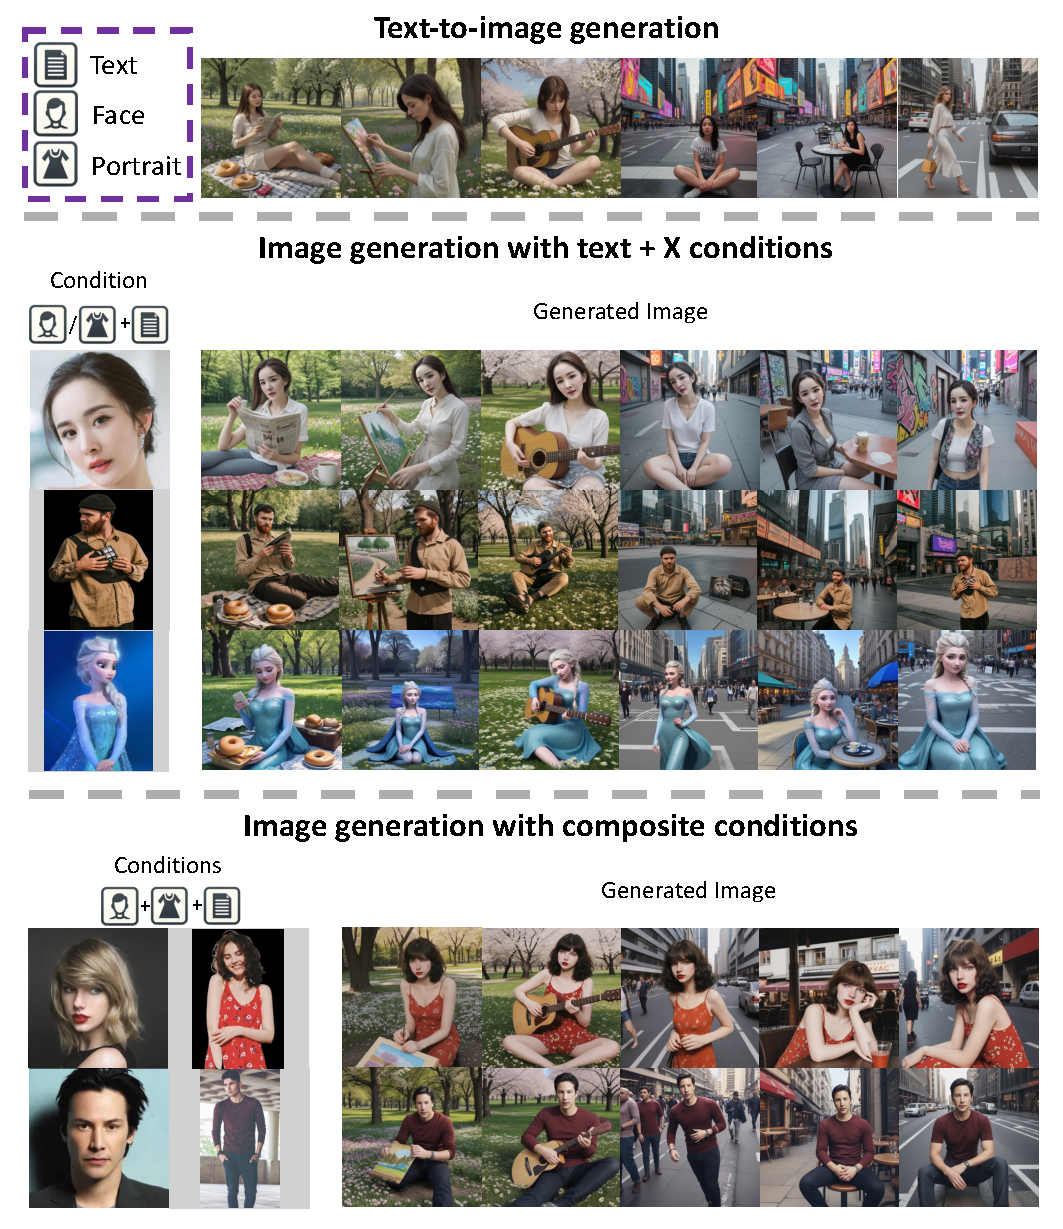
\includegraphics[width=0.9\textwidth]{images/final_visualization.pdf}
    \caption{Visualization for our EMMA's generalization ability under different conditions. Each column shares the same text prompts. We show three kinds of conditions. The first row shows the results when there is only the text condition. The second row shows the results under multi-modal conditions, such as text plus face conditions and text plus portrait conditions. The bottom row shows the results under composite conditions.}
    \label{fig:final_visualization}
\end{figure}

\subsection{Dataset settings}
\textbf{Common object dataset.} We also collect datasets for common objects. Following ELLA~\cite{hu2024ella}, we filter images collected from LAION~\cite{schuhmann2022laion} and COYO~\cite{kakaobrain2022coyo-700m} with an aesthetic score over 6 and a minimum short edge resolution of 512 pixels. We generate several random masks to provide guidance for the central object. In this way, we can train the model on a large-scale dataset. 

\textbf{Portrait dataset.} We collect an internal dataset containing 400K images for 100K human IDs. Our EMMA targeted at portrait generation is fine-tuned on the internal dataset for 200K iterations. The test dataset uses 32 portraits and 20 prompts for each portrait, which are crawled from the Unsplash website and available under a use license. 

\subsection{Training Details}

We train our model based on the principles established by the Stable Diffusion 1.5, with modifications to suit our experimental requirements. The model employs a half-precision floating-point (fp16) data type for efficiency. We only change the conditioner and keep all the other key components unchanged, including the pre-trained Variational Autoencoder (VAE), the noise scheduler, and the UNet.

All the experiments are done on 8 A100 GPUs. We manage a total training batch size of 256, with micro batches of 16 per GPU. We implement gradient clipping at a value of 1.0.
The optimizer of choice is AdamW, which is configured with a learning rate of 0.0001. This setup includes betas of 0.9 and 0.999, an epsilon value of 1e-8, and a weight decay of 0.01. The learning rate is adjusted linearly from 10\% to 100\% over the course of 1000 iterations.
For different conditions, we employ different feature extractors and datasets, which are detailed in the Appendix. 

\subsection{Personalized Story Diffusion } Given specific character information, our proposed EMMA could generate different images according to the text instruction, which makes it possible to generate results telling a story while maintaining character consistency. As shown in Figure~\ref{fig:story_diffusion}, we can generate a series of images based on a given portrait following text instructions. The persons could do various actions, which benefit from the strong instruction-following abilities of EMMA. 



\subsection{Quantitative Evaluation.}
\textbf{Style Conditioned Generation.} Following the evaluation settings of IP-Adapter~\cite{ye2023ip}, we evaluate the CLIP-T and CLIP-I scores of all methods on the COCO validation set. There are 5000 prompts in the validation set. We generate four images for each prompt as described in IP-Adapter~\cite{ye2023ip}.

\textbf{Portrait Generation.} We collect a dataset of portraits and construct 20 human action prompts based on the ActivityNet validation set. Building on this, we tested the generation capabilities of various subject-driven image generation methods and assessed the scores using the CLIP-T score and the DINO score metrics. Results are shown in Table~\ref{tab:main_table}, and our proposed EMMA achieves the highest score against previous methods. 

\textbf{Seperable Gate mechanism.} As shown in Table~\ref{tab:style_comparison}, we compare EMMA models trained under style conditions with and without separated gates. The EMMA with separated gates shows better performance, which is because such a design introduces finer control over different token embeddings. As observed in Figure~\ref{fig:gate_vis}, different tokens play different roles given specific conditions. Without the separated gates, the generated results will easily be influenced by unrelated token embeddings. 

\subsection{Visualization} 
\textbf{Different Conditions for Portrait Creation.} We have presented a variety of portrait generation outcomes. As seen in Figure \ref{fig:final_visualization}, our approach excels in maintaining key image elements like clothing and adheres closely to textual instructions. The top row illustrates the output of text-to-image generation, depicting a woman engaged in various activities across different settings. The middle row displays results from multi-modal image generation, where additional conditions such as facial or portrait traits yield images of a character that align with given instructions. The bottom row presents composite condition image generation, where we can produce images that follow instructions while retaining facial features from one image and portrait elements from another.


\textbf{Gate value visualization.} 
In our proposed EMMA, the gate design is a crucial module that enables free combination within our model. This design introduces an increased number of model parameters, enhancing the model's expressive capabilities. Furthermore, we observe a distinctive distribution of token indices of the significant gated values across various models. This unique pattern of token index distribution is crucial for the adaptability of our method, enabling flexible and unrestricted model integration. The visualization result is shown in Figure~\ref{fig:gate_vis}. 




\begin{figure}[t]
    \centering
    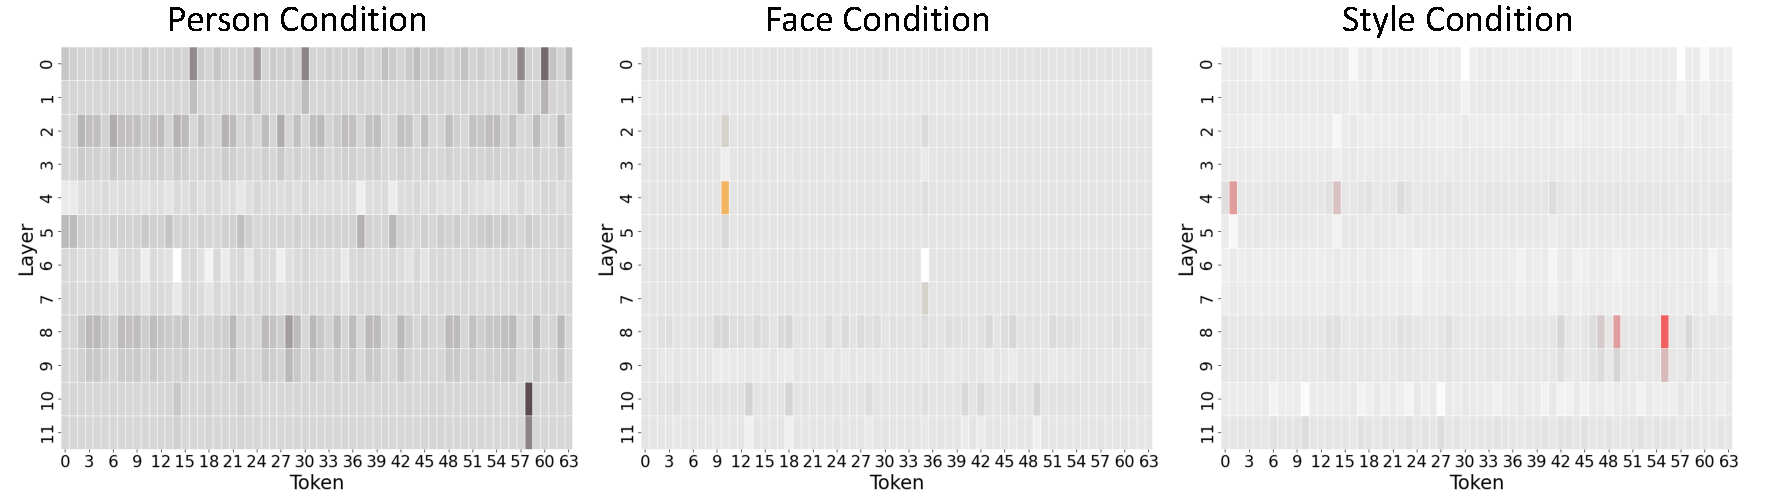
\includegraphics[width=0.95\textwidth]{images/token_visualization.pdf}
    \caption{Visualization for gate values under different conditions. The horizontal axis is the token index, while the vertical axis is the depth of the Layer. We found that the gate values show sparsity features in different layers. We also found that models trained under different conditions pay attention to different tokens, which is the basis of module composition.}
    \label{fig:gate_vis}
\end{figure}





